\section{Experiments}
\label{sec:experiments}

\subsection{Frozen Evaluation Design}
\label{sec:experimental-design}

The evaluation used a paired design frozen before Test outcomes were accessed
(hereafter, pre-Test-frozen). Protocol v2 and its first amendment fixed the
models, methods, scenarios, seeds, controller, endpoint, and analysis rule.
Three later amendments authorized continuation subject to balance constraints to
complete the matrix after partial execution but did not change those design
fields. The
content-addressed evidence snapshot \texttt{f4ab41daacf3} contains all 160
planned cells. No cell was excluded, and no completed cell was reissued while
creating the snapshot.

We evaluated ShiftMem and the lexical retrieval baseline with provider-hosted
DeepSeek-V3.2 and MiniMax-M2.5 through SiliconFlow. Test-ID comprised stable,
demand-jump, gradual-demand, and supply-delay scenarios. Test-OOD comprised
periodic recurrence, a Poisson demand jump, a transient demand excursion, and an
early combined demand-and-supply shift. Each scenario used five environment
seeds and 150 simulated days. Table~\ref{tab:frozen-design} summarizes the
matrix. The inference target is the tested provider deployments, not either
model family in the abstract.

\begin{table}[t]
  \caption{\textbf{Frozen held-out evaluation design.} The primary population
  excludes the stable scenario.}
  \label{tab:frozen-design}
  \centering
  \small
  \setlength{\tabcolsep}{3pt}
  \renewcommand{\arraystretch}{1.08}
  \begin{tabular}{@{}p{0.27\columnwidth}p{0.66\columnwidth}@{}}
    \toprule
    Component & Frozen setting \\
    \midrule
    Models & DeepSeek-V3.2; MiniMax-M2.5 \\
    Methods & ShiftMem; lexical retrieval baseline \\
    Scenarios & 4 Test-ID; 4 Test-OOD \\
    Seeds & 5 per scenario \\
    Full matrix & 160 complete cells \\
    Primary observations & 70 model-specific pairs in 35 environment clusters \\
    Endpoint & 30-day oracle-relative cost gap; $\Delta<0$ favors ShiftMem \\
    \bottomrule
  \end{tabular}
\end{table}

The primary analysis population excluded the stable scenario and contained 70
model-specific paired observations. Each pair matched on split, scenario, model
deployment, and environment seed and contained one run per method. The two
model-specific pairs for a common scenario and seed shared deterministic demand
and calendar-indexed supply streams. The 70 observations therefore formed 35 environment clusters
rather than 70 independent environment replicates. There was no independent
replication of stochastic LLM output.

\subsection{Endpoint and Statistical Analysis}
\label{sec:statistical-analysis}

The serialized primary endpoint was
\texttt{post\_shift\_cumulative\_regret\_30}, reported as the 30-day
oracle-relative cost gap over the first 30 complete days beginning at the
declared shift day. The Oracle was a parameter-aware base-stock heuristic, not a
proven optimum. For paired unit $i$, its common term cancels from the method
contrast:
\begin{equation}
\begin{split}
 \Delta_i&=(C_i^{\mathrm{Shift}}-C_i^{\mathrm{Oracle}})
 -(C_i^{\mathrm{Lex}}-C_i^{\mathrm{Oracle}})\\
 &=C_i^{\mathrm{Shift}}-C_i^{\mathrm{Lex}}.
\end{split}
 \label{eq:primary-contrast}
\end{equation}
Negative $\Delta_i$ favors ShiftMem. We report the mean difference
$\bar\Delta$, sample standard deviation $s_\Delta$, a nominal 95\% interval for
the mean difference, and paired standardized effect
\begin{equation}
 \mathrm{CI}_{95}=\bar\Delta\pm c_{.975,n-1}
 \frac{s_\Delta}{\sqrt n},\qquad d_z=\frac{\bar\Delta}{s_\Delta}.
 \label{eq:effect-summary}
\end{equation}
The frozen critical-value routine used tabulated values through 30 degrees of
freedom and 1.96 thereafter. We also report $n$ and ShiftMem wins, ties, and
losses, defined by negative, zero, and positive paired differences.

For sample skewness $g_1$ and kurtosis $g_2$, the normality diagnostic used
\begin{equation}
 J_n=\frac{n}{6}\left[g_1^2+\frac{(g_2-3)^2}{4}\right],
 \qquad p_N=\exp(-J_n/2).
 \label{eq:normality-diagnostic}
\end{equation}
A severe outlier was flagged when
$\max_i|\Delta_i-\operatorname{median}(\Delta)|>6\operatorname{MAD}(\Delta)$.
When MAD was zero, any nonzero deviation triggered the flag. The prespecified
rule selected a paired $t$-test when $p_N\geq0.05$ and no severe-outlier flag
was raised; otherwise, it selected a two-sided Wilcoxon signed-rank test. Nominal
mean intervals were retained under either test. A selected Wilcoxon $p$-value
therefore does not test the mean estimand directly. The split analysis was
prespecified. Model and scenario decompositions were descriptive. Their
$p$-values were unadjusted.

The frozen decision rule supported the ShiftMem-advantage hypothesis only when
the mean difference was negative and the selected two-sided test gave $p<0.05$.

The frozen primary calculation nevertheless treated the 70 model-specific
differences as inferential observations. Their clustering violates the
independence assumption, so the nominal interval and $p$-value are not calibrated
for cluster-level inference. The split-level nominal intervals and $p$-values
inherit this limitation and are reported as descriptive protocol-frozen
summaries. We retained the frozen calculation unchanged and added a post-hoc
sensitivity that averaged model effects within each of the 35 clusters and
retained seven fixed scenario strata with five environment-seed clusters each.
Within each stratum, the sensitivity resampled clusters with replacement 50,000
times and used the 2.5th and 97.5th percentiles of the equal-scenario mean. It
also applied a two-sided Monte Carlo cluster sign-flip test to that mean under
sign exchangeability of cluster differences. For the deployment contrast, we
formed the within-cluster DeepSeek-minus-MiniMax method-effect difference and
applied the same stratified procedures. Each bootstrap and sign-flip procedure
used 50,000 draws. The overall bootstrap and sign-flip seeds were 20260723 and
20260724; the deployment-contrast seeds were 20260733 and 20260734. The custom
dependency-light routines ran under CPython 3.12.7 and NumPy 2.5.1. Figures used
Matplotlib 3.11.0. Analysis code was SHA-256-bound.

\subsection{Primary Effect}
\label{sec:primary-result}

The primary analysis did not support an improvement by ShiftMem. Across 70
pairs, the mean difference between ShiftMem and the lexical retrieval baseline
was $+45.44$ (nominal 95\% mean CI
$[-2.72,93.60]$; $s_\Delta=205.59$; $d_z=0.221$). The frozen rule selected the
Wilcoxon normal approximation ($W=716$, two-sided $p=0.203$). ShiftMem won 25
pairs, tied 11, and lost 34. Here $W$ is the smaller of the positive and
negative rank sums after removing zero differences and averaging tied ranks.
The normal approximation used continuity correction. The prespecified decision
rule therefore did not support the prespecified ShiftMem-advantage hypothesis,
and the point estimate was unfavorable to ShiftMem. Given the dependence
limitation, neither the interval nor the test establishes equivalence or
intrinsic failure of the conditional memory lifecycle.

The post-hoc clustered sensitivity pointed in the same unfavorable
direction. Its estimate remained $+45.44$, with a cluster-bootstrap 95\% CI of
$[11.26,79.09]$ and sign-flip $p=0.041$ across 35 clusters. This post-hoc result
does not replace the prespecified analysis or convert the original advantage
hypothesis into a supported claim. In this sensitivity analysis, accounting for
shared environment streams did not recover a favorable average effect.

\begin{figure*}[t]
  \centering
  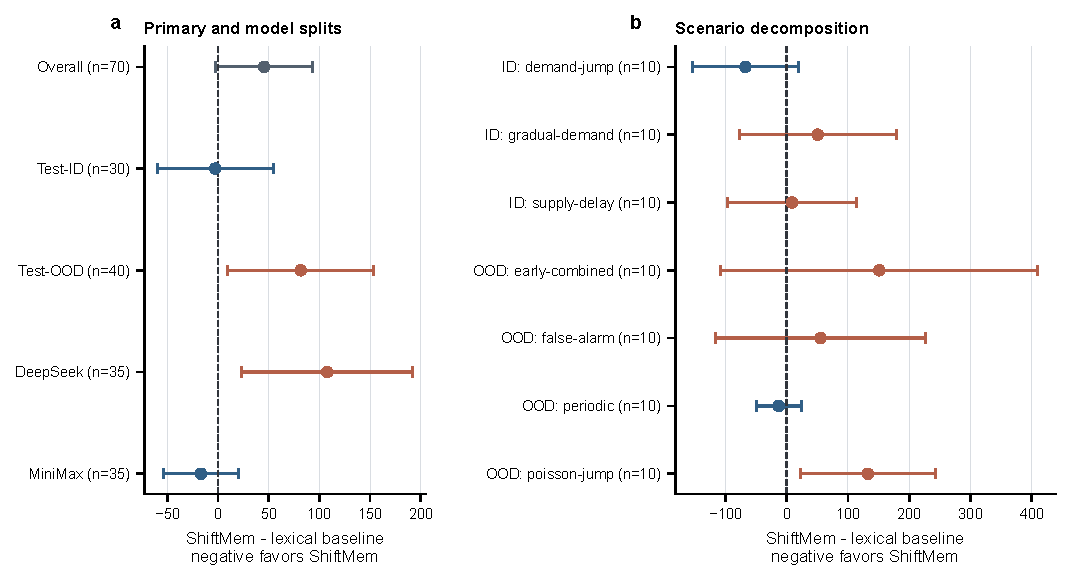
\includegraphics[width=\textwidth]{figures/figure_2_effect_forest.pdf}
  \caption{\textbf{Differences between ShiftMem and the lexical retrieval
  baseline in the 30-day
  oracle-relative cost gap.} Negative values favor ShiftMem. Points denote mean
  paired differences; bars are nominal 95\% mean-difference intervals from the
  frozen summary routine. \textbf{a}, The overall row is the prespecified
  dependence-limited primary calculation ($n=70$ model-specific pairs in 35
  environment clusters). Its two-sided hypothesis test used the selected
  Wilcoxon signed-rank test, which targets a different quantity from the
  displayed mean interval.
  Test-ID and Test-OOD are the prespecified descriptive split. Model rows are
  unadjusted descriptive decompositions. \textbf{b}, Scenario decompositions are
  descriptive and unadjusted (ten model-specific pairs in five environment
  clusters each). These subgroup results do not establish generalizable effect
  modification by deployment or scenario. Source data are provided
  in the evidence package.}
  \label{fig:effects}
\end{figure*}

\subsection{Split, Model, and Scenario Heterogeneity}
\label{sec:heterogeneity}

The Test-ID and Test-OOD point estimates had opposite signs. Test-ID had a mean
point estimate near zero ($\bar\Delta=-2.67$, nominal 95\% mean CI
$[-60.17,54.82]$, 30 model-specific pairs in 15 environment clusters, paired-$t$
$p=0.925$); its wide interval does not establish equivalence. Test-OOD had an
unfavorable point estimate ($+81.53$, nominal 95\% mean CI $[9.50,153.56]$, 40
model-specific pairs in 20 environment clusters, Wilcoxon $p=0.093$).
The Test-OOD mean interval excluded zero while the rank-based test did not reject.
These summaries target different quantities. Neither split result supports a
universal claim about in- or out-of-distribution behavior.

The two provider-hosted model deployments also showed opposite descriptive
directions. DeepSeek had $\bar\Delta=+107.73$ (nominal 95\% mean CI
$[23.09,192.37]$, 35 environment-level paired differences, unadjusted Wilcoxon
$p=0.023$), whereas MiniMax had $\bar\Delta=-16.85$ (nominal 95\% mean CI
$[-53.91,20.22]$, 35 environment-level paired differences, unadjusted paired-$t$
$p=0.379$).
The post-hoc DeepSeek-minus-MiniMax method-effect contrast was $+124.58$
(cluster-bootstrap 95\% CI $[38.59,216.05]$, unadjusted sign-flip $p=0.015$).
No multiplicity correction was applied across the exploratory analyses. The
unadjusted post-hoc contrast suggests effect modification between these two
tested deployments, but only two deployments and no independent LLM replications
were available. It therefore does not establish generalizable effect
modification across deployments or model families.

Scenario means ranged from $-67.38$ for the Test-ID demand jump to $+151.24$
for the early combined OOD shift (Fig.~\ref{fig:effects}b). Each estimate used
only ten model-specific pairs in five environment clusters, was unadjusted, and
had generally wide uncertainty. We therefore report the set as a decomposition
rather than ranking scenarios. The mean ShiftMem-minus-baseline difference in
stable-environment total cost was $+15.86$ (nominal 95\% mean CI
$[-184.37,216.09]$, ten model-specific pairs in five environment clusters).
Because no non-inferiority margin was frozen, this result establishes neither
equivalence nor absence of degradation.

Table~\ref{tab:effects} reports the complete aggregate effect set with evidence
status labels.
\begin{table*}[t]
  \centering
  \scriptsize
  \caption{\textbf{Complete primary, descriptive, and post-hoc effect
  summaries.} Differences are ShiftMem minus the lexical retrieval baseline;
  negative values favor ShiftMem. Except for the two post-hoc cluster rows,
  intervals are nominal mean-difference intervals from the frozen routine and
  are not calibrated for cluster-level inference. W/T/L denotes ShiftMem wins,
  ties, and losses.}
  \label{tab:effects}
  \resizebox{\textwidth}{!}{%
  \begin{tabular}{@{}lrrrrllrl@{}}
    \toprule
    Analysis & $n$ & $\bar\Delta$ & 95\% CI & $d_z$ & W/T/L & Test & $p$ & Evidence status \\
    \midrule
    Overall & 70 & 45.44 & $[-2.72,93.60]$ & .221 & 25/11/34 & Wilcoxon-N & .2034 & Prespecified, dependence-limited \\
    Test-ID & 30 & -2.67 & $[-60.17,54.82]$ & -.017 & 12/6/12 & Paired $t$ & .9249 & Prespecified descriptive \\
    Test-OOD & 40 & 81.53 & $[9.50,153.56]$ & .351 & 13/5/22 & Wilcoxon-N & .0932 & Prespecified descriptive \\
    DeepSeek & 35 & 107.73 & $[23.09,192.37]$ & .422 & 9/6/20 & Wilcoxon-N & .0232 & Unadjusted descriptive \\
    MiniMax & 35 & -16.85 & $[-53.91,20.22]$ & -.151 & 16/5/14 & Paired $t$ & .3793 & Unadjusted descriptive \\
    ID: demand jump & 10 & -67.38 & $[-153.83,19.07]$ & -.557 & 6/1/3 & Paired $t$ & .1117 & Descriptive subgroup \\
    ID: gradual demand & 10 & 50.62 & $[-77.60,178.84]$ & .282 & 2/4/4 & Paired $t$ & .3951 & Descriptive subgroup \\
    ID: supply delay & 10 & 8.74 & $[-96.67,114.15]$ & .059 & 4/1/5 & Paired $t$ & .8554 & Descriptive subgroup \\
    OOD: early combined & 10 & 151.24 & $[-107.60,410.08]$ & .418 & 4/0/6 & Paired $t$ & .2189 & Descriptive subgroup \\
    OOD: transient excursion & 10 & 55.26 & $[-116.55,227.07]$ & .230 & 3/2/5 & Wilcoxon-E & .7422 & Descriptive subgroup \\
    OOD: periodic & 10 & -12.94 & $[-49.87,23.99]$ & -.251 & 4/2/4 & Wilcoxon-E & .6406 & Descriptive subgroup \\
    OOD: Poisson jump & 10 & 132.56 & $[22.08,243.04]$ & .858 & 2/1/7 & Paired $t$ & .0238 & Descriptive subgroup \\
    Stable total cost & 10 & 15.86 & $[-184.37,216.09]$ & .057 & 5/2/3 & Wilcoxon-E & 1.000 & Descriptive, different endpoint \\
    Clustered overall & 35 & 45.44 & $[11.26,79.09]$ & -- & -- & Sign flip & .0414 & Post-hoc sensitivity \\
    DeepSeek--MiniMax & 35 & 124.58 & $[38.59,216.05]$ & -- & -- & Sign flip & .0154 & Post-hoc, unadjusted \\
    \bottomrule
  \end{tabular}}
\end{table*}


\subsection{Recovery and System Reliability}
\label{sec:reliability-results}

Recovery was defined from rolling cost rather than the primary cost-gap
endpoint. A cell recovered when the absolute difference between its seven-day
rolling total cost and the paired Oracle's rolling cost did not exceed 10\% of
the Oracle value for seven consecutive overlapping window endpoints.
Otherwise, it was right-censored at the final day. Recovery occurred in 61 of
140 applicable cells: 32 of 70 for ShiftMem and 29 of 70 for the lexical
retrieval baseline. These counts are descriptive and do not account for censoring through
a survival model.

Reliability burden was part of the evaluated system rather than an exclusion
criterion. The 160 cells recorded 5,176 reviews and 6,189 attempts. Of these
attempts, 1,680 were coded as failed or invalid (27.1\%); this aggregate is stored
as \texttt{parse\_failures} and includes provider exceptions as well as JSON or
schema failures. After the permitted retry, 667
reviews retained the previous strategy (12.9\%). Cell records contained 28.72M
input and 2.08M output tokens. Burden varied more strongly by model than by
memory method: failed/invalid-attempt rates were 9.8\% for DeepSeek and 40.9\%
for MiniMax, while retained-strategy rates were 4.6\% and 21.1\%, respectively.
Figure~\ref{fig:reliability} reports the split--model--method groups without
inferential error bars.

\begin{figure*}[t]
  \centering
  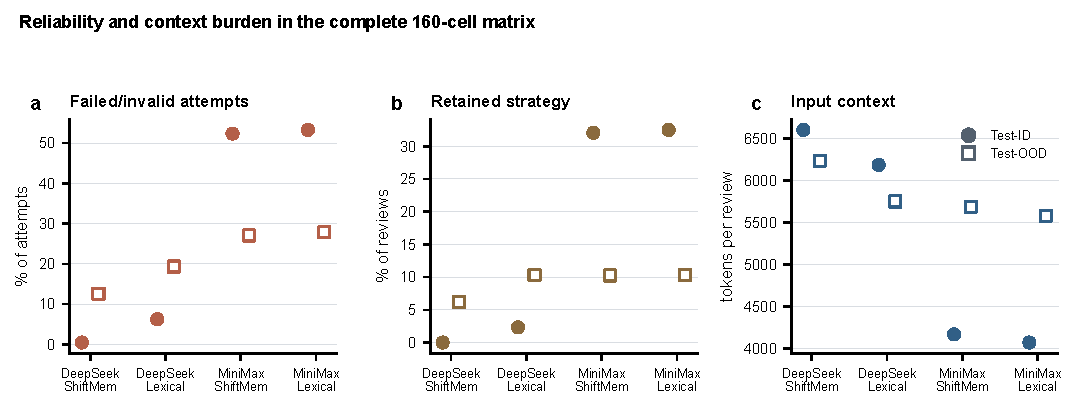
\includegraphics[width=\textwidth]{figures/figure_3_reliability.pdf}
  \caption{\textbf{Reliability and input-context burden across the 160-cell
  matrix.} Filled circles denote Test-ID and open squares denote Test-OOD. Each
  point aggregates 20 cells for one split--model--method combination.
  \textbf{a}, Cell-coded failed or invalid attempts as a percentage of
  cell-recorded attempts. This category includes provider exceptions and
  structured-output failures. \textbf{b}, Reviews that retained the previous
  valid strategy as a percentage of strategy reviews. \textbf{c}, Cell-recorded input tokens per
  review. These aggregate rates are descriptive and do not identify a causal
  effect of reliability on inventory outcomes. Source data are provided in the
  evidence package.}
  \label{fig:reliability}
\end{figure*}

Table~\ref{tab:reliability} reports the corresponding reliability and context
totals.
\begin{table*}[t]
  \centering
  \scriptsize
  \caption{\textbf{Reliability, context, and recovery by split, deployment,
  and method.} Each row aggregates 20 cells. Failed/invalid counts include
  provider exceptions and invalid structured outputs and use cell-recorded
  attempts as the denominator. Fallbacks use reviews as the denominator. Token
  totals are in millions. Recovery is descriptive and excludes stable cells.}
  \label{tab:reliability}
  \resizebox{\textwidth}{!}{%
  \begin{tabular}{@{}lllrrrrrrr@{}}
    \toprule
    Split & Deployment & Method & Attempts & Failed/invalid & Reviews & Fallbacks & Input M & Output M & Recovered \\
    \midrule
    Test-ID & DeepSeek & ShiftMem & 681 & 3 (0.4\%) & 678 & 0 (0.0\%) & 4.477 & 0.068 & 8/15 \\
    Test-ID & DeepSeek & Lexical & 625 & 39 (6.2\%) & 600 & 14 (2.3\%) & 3.711 & 0.061 & 7/15 \\
    Test-ID & MiniMax & ShiftMem & 966 & 506 (52.4\%) & 677 & 217 (32.1\%) & 2.820 & 0.413 & 13/15 \\
    Test-ID & MiniMax & Lexical & 867 & 462 (53.3\%) & 600 & 195 (32.5\%) & 2.441 & 0.359 & 10/15 \\
    Test-OOD & DeepSeek & ShiftMem & 761 & 96 (12.6\%) & 709 & 44 (6.2\%) & 4.422 & 0.064 & 4/20 \\
    Test-OOD & DeepSeek & Lexical & 667 & 129 (19.3\%) & 600 & 62 (10.3\%) & 3.450 & 0.056 & 6/20 \\
    Test-OOD & MiniMax & ShiftMem & 876 & 237 (27.1\%) & 712 & 73 (10.3\%) & 4.049 & 0.579 & 7/20 \\
    Test-OOD & MiniMax & Lexical & 746 & 208 (27.9\%) & 600 & 62 (10.3\%) & 3.349 & 0.484 & 6/20 \\
    \bottomrule
  \end{tabular}}
\end{table*}


The append-only provider journals retained 4,558 successful responses and 1,705
terminal failed attempts. Their 6,263 terminal attempts exceed the 6,189
cell-recorded attempts by 74 because interrupted or otherwise non-final attempts
remain in the journals.
Estimated successful-response cost was CNY 108.49. The separate failed-attempt
reservation ledger recorded CNY 93.88. Neither quantity is the official provider
bill, which remains unreconciled.

The evidence manifest also documents 161 erroneous metadata indicators of
Test-outcome access introduced by a raw serializer default. It preserves the
source bytes and reports no effect on numeric outcomes.

\subsection{Exploratory Diagnostics and Limitations}
\label{sec:diagnostic-limits}

Post-hoc burden correlations were small. Across 70 pairs, correlations between
relative burden and the paired endpoint ranged from $-0.134$ to $-0.055$ across
Pearson and Spearman
summaries for failed/invalid attempts, fallbacks, and journal-recorded provider
failures. These post-hoc associations have no reported inferential $p$-values
and do not identify mediation or causality.

Execution order remains an unresolved limitation. All 70 pairs ran the lexical
retrieval baseline before ShiftMem, and the journals contain append order rather
than wall-clock timestamps. The early and late halves had mean differences of
$+58.58$ and $+32.30$. Correlations with execution position were 0.159
(Pearson) and 0.175 (Spearman). These diagnostics do not remove confounding by
method order or provider drift. A valid follow-up must randomize or
counterbalance execution order.

The held-out evaluation tested one synthetic single-item environment family, two
provider deployments, five environment seeds per scenario, one lexical retrieval
baseline, and no independent LLM-output replications. It did not formally
compare ShiftMem with a broader set of memory baselines, test
dormancy/reactivation through ablation, or compare the Page--Hinkley trigger with
an LLM-only detector. Stable-scenario performance remained descriptive because
no non-inferiority margin was frozen. The results therefore evaluate the two
deployed systems under the specified protocol. They do not identify the causal
value of an individual lifecycle component or establish general memory
superiority. Model identifiers and the output-token cap were frozen, but the
complete resolved provider request settings and provider-side defaults for
omitted decoding controls were not persisted. Exact API-level replication is
therefore limited to the recorded fields and raw responses.
